% Springer/Quarto PDF header includes.
%
% Quarto owns execution, assembly, cross-references, and bibliography wiring.
% Springer remains the PDF class contract through documentclass: SNmono in
% _quarto.yml. Keep publisher-specific LaTeX here rather than in chapters.

\usepackage{type1cm}
\usepackage{array}
\usepackage{float}
\usepackage{placeins}
\usepackage{needspace}
\usepackage[bottom]{footmisc}
\usepackage{xcolor}
\usepackage{fontawesome5}
\usepackage[most]{tcolorbox}
\usepackage{tikz}
\usetikzlibrary{arrows.meta,calc,positioning,shapes.geometric}
\usepackage{newtxtext}
\usepackage[varvw]{newtxmath}
\renewcommand{\ttdefault}{cmtt}

\bibpunct{(}{)}{;}{a}{,}{,}
\SuppressSpringerImprint
\SetArchTwoPreviewVersion{Preview v0.2.0}

\definecolor{archtwoink}{HTML}{20252B}
\definecolor{archtwomuted}{HTML}{59636D}
\definecolor{archtwoblue}{HTML}{1F5F7A}
\definecolor{archtwobluefill}{HTML}{EEF7FB}
\definecolor{archtwogreen}{HTML}{4B7F52}
\definecolor{archtwogreenfill}{HTML}{F1F8F0}
\definecolor{archtwoorange}{HTML}{A9671E}
\definecolor{archtwoorangefill}{HTML}{FFF6E8}
\definecolor{archtwoline}{HTML}{9AA8B5}
\definecolor{archtwopanel}{HTML}{F7FAFB}
\definecolor{archtwogrid}{HTML}{E2E8ED}
\definecolor{archtwoevidence}{HTML}{7E6AA8}
\definecolor{archtwoevidencefill}{HTML}{F4F1FA}
\definecolor{archtwoodanger}{HTML}{C44E52}
\definecolor{archtwoodangerfill}{HTML}{F8EAEA}

\newcommand{\ArchTwoCoverMotif}{%
  \begingroup
  \sffamily
  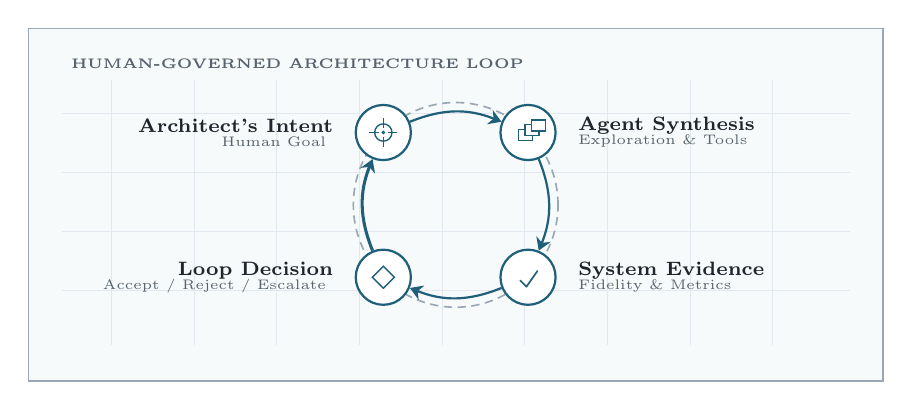
\begin{tikzpicture}[
    x=1cm,
    y=1cm,
    >=Stealth,
    arrow/.style={-{Stealth[length=4.5pt,width=5.5pt]}, line width=0.8pt, draw=archtwoblue},
    feedback/.style={-{Stealth[length=4.5pt,width=5.5pt]}, line width=1.1pt, draw=archtwoblue}
  ]
    \fill[archtwopanel] (0,0) rectangle (10.85,4.48);
    \draw[archtwoline, line width=0.6pt] (0,0) rectangle (10.85,4.48);
    \foreach \x in {1.05,2.10,3.15,4.20,5.25,6.30,7.35,8.40,9.45} {
      \draw[archtwogrid, line width=0.25pt] (\x,0.46) -- (\x,3.82);
    }
    \foreach \y in {1.15,1.90,2.65,3.40} {
      \draw[archtwogrid, line width=0.25pt] (0.42,\y) -- (10.43,\y);
    }

    \node[anchor=north west, font=\tiny\bfseries, text=archtwomuted] at (0.42,4.22)
      {HUMAN-GOVERNED ARCHITECTURE LOOP};

    \coordinate (center) at (5.425, 2.24);

    \draw[archtwoline, line width=0.6pt, dash pattern=on 3pt off 2pt] (center) circle (1.3cm);

    \coordinate (intent) at (4.506, 3.159);
    \coordinate (synthesis) at (6.344, 3.159);
    \coordinate (evidence) at (6.344, 1.321);
    \coordinate (decide) at (4.506, 1.321);

    \node[circle, draw=archtwoblue, fill=white, line width=0.8pt, minimum size=0.7cm] (N-intent) at (intent) {};
    \node[circle, draw=archtwoblue, fill=white, line width=0.8pt, minimum size=0.7cm] (N-synthesis) at (synthesis) {};
    \node[circle, draw=archtwoblue, fill=white, line width=0.8pt, minimum size=0.7cm] (N-evidence) at (evidence) {};
    \node[circle, draw=archtwoblue, fill=white, line width=0.8pt, minimum size=0.7cm] (N-decide) at (decide) {};

    % 1. Intent Glyph (Target/Crosshair)
    \draw[archtwoblue, line width=0.5pt] (intent) circle (0.11);
    \fill[archtwoblue] (intent) circle (0.025);
    \draw[archtwoblue, line width=0.45pt] ($(intent)+(0,0.18)$) -- ($(intent)+(0,0.06)$);
    \draw[archtwoblue, line width=0.45pt] ($(intent)+(0,-0.18)$) -- ($(intent)+(0,-0.06)$);
    \draw[archtwoblue, line width=0.45pt] ($(intent)+(0.18,0)$) -- ($(intent)+(0.06,0)$);
    \draw[archtwoblue, line width=0.45pt] ($(intent)+(-0.18,0)$) -- ($(intent)+(-0.06,0)$);

    % 2. Synthesis Glyph (Stacked Rectangles)
    \draw[archtwoblue, line width=0.45pt, fill=white] ($(synthesis)+(-0.12,-0.10)$) rectangle ++(0.18,0.14);
    \draw[archtwoblue, line width=0.45pt, fill=white] ($(synthesis)+(-0.04,-0.04)$) rectangle ++(0.18,0.14);
    \draw[archtwoblue, line width=0.45pt, fill=white] ($(synthesis)+(0.04,0.02)$) rectangle ++(0.18,0.14);

    % 3. Evidence Glyph (Checkmark)
    \draw[archtwoblue, line width=0.6pt, line cap=round, line join=round] ($(evidence)+(-0.10,-0.04)$) -- ($(evidence)+(-0.02,-0.12)$) -- ($(evidence)+(0.12,0.08)$);

    % 4. Decision Glyph (Diamond)
    \draw[archtwoblue, line width=0.5pt, fill=white] (decide) ++(0,0.14) -- ++(0.14,-0.14) -- ++(-0.14,-0.14) -- ++(-0.14,0.14) -- cycle;

    \draw[arrow] (N-intent) to[bend left=22] (N-synthesis);
    \draw[arrow] (N-synthesis) to[bend left=22] (N-evidence);
    \draw[arrow] (N-evidence) to[bend left=22] (N-decide);
    \draw[feedback] (N-decide) to[bend left=22] (N-intent);

    \node[left=0.15cm of N-intent, font=\scriptsize\bfseries, text=archtwoink, align=right] (L-intent) {
      Architect's Intent \\[-3pt] \tiny\color{archtwomuted}\textnormal{Human Goal}
    };

    \node[right=0.15cm of N-synthesis, font=\scriptsize\bfseries, text=archtwoink, align=left] (L-synthesis) {
      Agent Synthesis \\[-3pt] \tiny\color{archtwomuted}\textnormal{Exploration \& Tools}
    };

    \node[right=0.15cm of N-evidence, font=\scriptsize\bfseries, text=archtwoink, align=left] (L-evidence) {
      System Evidence \\[-3pt] \tiny\color{archtwomuted}\textnormal{Fidelity \& Metrics}
    };

    \node[left=0.15cm of N-decide, font=\scriptsize\bfseries, text=archtwoink, align=right] (L-decide) {
      Loop Decision \\[-3pt] \tiny\color{archtwomuted}\textnormal{Accept / Reject / Escalate}
    };

  \end{tikzpicture}%
  \endgroup
}

\makeatletter
\def\@maketitle{%
  \thispagestyle{empty}%
  \begingroup
    \parindent=\z@
    \color{archtwoink}%
    \begin{tikzpicture}[remember picture,overlay]
      \fill[archtwopanel] (current page.north west)
        rectangle ([yshift=-0.58in]current page.north east);
      \fill[archtwoblue] ([xshift=0.76in,yshift=-0.58in]current page.north west)
        rectangle ([xshift=0.82in,yshift=1.12in]current page.south west);
      \draw[archtwogrid, line width=0.45pt]
        ([xshift=0.82in,yshift=-0.58in]current page.north west) --
        ([yshift=-0.58in]current page.north east);
    \end{tikzpicture}%
    \vspace*{-0.56in}%
    {\large\@author\par}%
    \vspace{0.10in}%
    {\small\bfseries\color{archtwoblue}PREVIEW EDITION\par}%
    \vspace{0.62in}%
    {\color{archtwoblue}\rule{0.78in}{1.2pt}\par}%
    \vspace{0.18in}%
    {\fontsize{35}{39}\selectfont\bfseries\@title\par}%
    \vspace{0.28in}%
    \if!\@subtitle!\else
      {\Large\color{archtwomuted}\@subtitle\par}%
      \vspace{0.62in}%
    \fi
    \ArchTwoCoverMotif\par
    \vfill
    {\color{archtwoline}\rule{\textwidth}{0.45pt}\par}%
    \vspace{0.14in}%
    {\small\bfseries Work in progress\par}%
    \vspace{0.10in}%
    {\small\color{archtwomuted}\ArchTwoPreviewVersion\ for the ISCA 2026 Architecture 2.0 workshop.\par}%
    \ifx\@date\@empty\else
      \vspace{0.10in}%
      {\small\color{archtwomuted}\@date\par}%
    \fi
    \vspace*{0.40in}%
  \endgroup
}

\def\@makechapterhead#1{{\parindent\z@\raggedright\normalfont
  \hyphenpenalty \@M
  \interlinepenalty\@M
  \if@chapnum
     \chapnumsize\chapnumstyle
     \@chapapp\ \thechapter\thechapterend\par
     \vskip 2\p@
  \fi
  \chapsize\chapstyle
  \ignorespaces#1\par\nobreak
  \vskip 8\p@
  {\color{archtwoblue}\rule{0.72in}{1.0pt}\par}%
  \processchapsubtit
  \processchapauthor
  \processmotto
  \ifdim\pagetotal>140\p@
     \vskip 11\p@
  \else
     \@tempdima=140\p@\advance\@tempdima by-\pagetotal
     \vskip\@tempdima
  \fi}}

\def\@makeschapterhead#1{{\parindent \z@ \raggedright\normalfont
  \hyphenpenalty \@M
  \interlinepenalty\@M
  \chapsize\chapstyle
  \ignorespaces#1\par\nobreak
  \vskip 8\p@
  {\color{archtwoblue}\rule{0.72in}{1.0pt}\par}%
  \processmotto
  \ifdim\pagetotal>140\p@
     \vskip 11\p@
  \else
     \@tempdima=140\p@\advance\@tempdima by-\pagetotal
     \vskip\@tempdima
  \fi}}

\def\ps@bchap{%
  \let\@oddhead\@empty\let\@evenhead\@empty
  \def\@oddfoot{\reset@font\small\color{archtwomuted}\ArchTwoPreviewVersion\hfil\thepage}%
  \let\@evenfoot\@oddfoot}

\def\ps@headings{\let\@mkboth\markboth
   \def\@oddfoot{\reset@font\scriptsize\color{archtwomuted}\ArchTwoPreviewVersion\hfil}%
   \def\@evenfoot{\reset@font\scriptsize\color{archtwomuted}\hfil Architecture 2.0}%
   \def\@evenhead{\runheadsize\runheadstyle\rlap{\thepage}\hfil
                  \leftmark}
   \def\@oddhead{\runheadsize\runheadstyle\rightmark\hfil
                  \llap{\thepage}}
   \def\chaptermark##1{\markboth{{\if@chapnum
      \thechapter\thechapterend\hskip\betweenumberspace\fi ##1}}{{\if@chapnum
      \thechapter\thechapterend\hskip\betweenumberspace\fi ##1}}}%
   \def\sectionmark##1{\markright{{\ifnum\c@secnumdepth>\z@
      \thesection\seccounterend\hskip\betweenumberspace\fi ##1}}}}
\makeatother

\newcolumntype{L}[1]{>{\raggedright\arraybackslash}p{#1}}

% Global table breathing room: applies to every tabular that does not set its
% own arraystretch. Wide tables keep their local \tabcolsep overrides.
\renewcommand{\arraystretch}{1.3}
\setlength{\tabcolsep}{4pt}

% Quarto PDF callouts emit tcolorbox environments and these color names.
% Keep the palette restrained so boxes read like manuscript aids, not slides.
\definecolor{quarto-callout-note-color}{HTML}{2A5B84}
\definecolor{quarto-callout-note-color-frame}{HTML}{7FA7C4}
\definecolor{quarto-callout-tip-color}{HTML}{3B6B3D}
\definecolor{quarto-callout-tip-color-frame}{HTML}{8DB98F}
\definecolor{quarto-callout-important-color}{HTML}{6E4B8B}
\definecolor{quarto-callout-important-color-frame}{HTML}{A993BF}
\definecolor{quarto-callout-warning-color}{HTML}{9A5A00}
\definecolor{quarto-callout-warning-color-frame}{HTML}{D6A64A}
\definecolor{quarto-callout-caution-color}{HTML}{8A2D2D}
\definecolor{quarto-callout-caution-color-frame}{HTML}{C78585}
